\documentclass[13pt]{beamer}
\usepackage{graphicx}
\usepackage[utf8]{inputenc}
\usepackage[skip=2pt,font=scriptsize]{caption}
\usepackage{algorithm}
\usepackage{algorithmic}

% Algorithms
\renewcommand{\algorithmicrequire}{\textbf{Input:}}
\renewcommand{\algorithmicensure}{\textbf{Output:}}
\algsetup{linenosize=\small}

% Captions
\captionsetup{labelformat=empty,labelsep=none}
\DeclareCaptionFormat{myformat}{#3}
\captionsetup[algorithm]{format=myformat}

% References
\usepackage{url}
\bibliographystyle{acm}
\setbeamertemplate{bibliography item}[triangle]

% Formatting
\usetheme{Singapore}
\usecolortheme{whale}

% Title Page
\title{The Sieve of Eratosthenes using MPI}
\author{Devin Delfino}
\institute{Comp 401: Senior Seminar}
\date{4/16/2015}

% Table of Contents
\setbeamertemplate{section in toc}[sections numbered]
\setbeamercolor{alerted text}{fg=blue}
\AtBeginSection[]
{
  \begin{frame}
    \frametitle{Outline}
    \tableofcontents[currentsection]
  \end{frame}
}

\begin{document}
% TITLE ------------------------------------------------
\frame{\titlepage}


% Table of Contents ------------------------------------------------
\begin{frame}
\frametitle{Outline}
\tableofcontents
\end{frame}

\section{The Sequential Algorithm} % ==========================================================================
% The Sequential Sieve ------------------------------------------------
\begin{frame}
\frametitle{The Sequential Algorithm}
	\begin{algorithm}[H]
        \small
        \caption{Merge}
        \begin{algorithmic}
          \REQUIRE Node* root\_A, Node* root\_B

          \IF{root\_A.key $\leq$ root\_B.key}
            \STATE root\_B.right\_sibling $\leftarrow$ root\_A.child
            \STATE root\_A.child $\leftarrow$ root\_B
            \STATE root\_B.parent $\leftarrow$ root\_A
            \RETURN root\_A
          \ELSE
            \STATE root\_A.right\_sibling $\leftarrow$ root\_B.child
            \STATE root\_B.child $\leftarrow$ root\_A
            \STATE root\_A.parent $\leftarrow$ root\_B
            \RETURN root\_B
          \ENDIF
        \end{algorithmic}
        \end{algorithm}
\end{frame}

\section{Parallel Programming and MPI} % ==========================================================================
% Parallel Programming Introduction ------------------------------------------------
\begin{frame}
\frametitle{Binomial Trees: Examples}
\begin{figure}
        \caption{Example: $k = 3$, $d = 2$}
        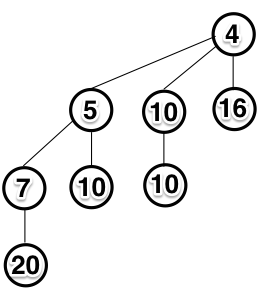
\includegraphics[height=3cm]{./img/order3.png}
      \end{figure}
\end{frame}

% MPI Introduction ------------------------------------------------
\begin{frame}
\frametitle{Binomial Trees: Examples}
\begin{figure}
        \caption{Example: $k = 3$, $d = 2$}
        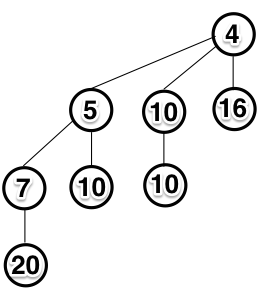
\includegraphics[height=3cm]{./img/order3.png}
      \end{figure}
\end{frame}

% Parallel Programming Design ------------------------------------------------
\begin{frame}
\frametitle{Parallel Programming Design}
\begin{figure}
        \caption{Example: $k = 3$, $d = 2$}
        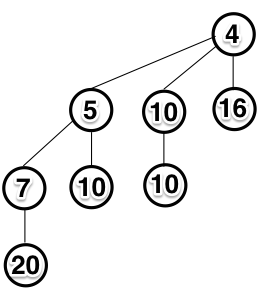
\includegraphics[height=3cm]{./img/order3.png}
      \end{figure}
\end{frame}

\section{The Parallel Algorithm} % ==========================================================================
% Block Allocation ------------------------------------------------
\begin{frame}
\frametitle{The Parallel Algorithm: Block Allocation}
  
\end{frame}

% Translating Sequential Algorithm ------------------------------------------------
\begin{frame}
\frametitle{The Parallel Algorithm: Developing Algorithm}
  
\end{frame}

\section{Sequential vs. Parallel Comparison} % ========================================================================
% Comparison: Seq vs. Par ------------------------------------------------
\begin{frame}
\frametitle{Sequential vs. Parallel}
  
\end{frame}

% References ------------------------------------------------
 \begin{frame}
  \frametitle{References}
  \nocite{*} 
  \bibliography{workscited}
\end{frame}

\end{document}